\section{Specifications}


\begin{table}[htbp]
\label{motor_specs}
\caption[Specifications of supported motors.]{Specifications of supported motors.}
\centering
\begin{tabular}{|l|c|c|}
\hline 
 & SMC2242 & SMC4242 \\ \hline 
Number of Motors: & 2 & 4 \\ \hline
Motor Type: & \multicolumn{2}{c|}{Bipolar Stepper Motor} \\ \hline
Motor Drive Voltage: & \multicolumn{2}{c|}{\unit[24]{V}} \\ \hline
Motor Current: & \multicolumn{2}{c|}{up to \unit[2.5]{A} peak or \unit[1.75]{A} RMS} \\ \hline
\end{tabular}
\end{table}

\newcolumntype{C}[1]{>{\centering\arraybackslash}p{#1}}
\begin{table}[htbp]
  \label{specs}
  \caption[Specifications of \productNumber ~\productName .]{Specifications of \productNumber ~\productName . With $V_{\textrm{Supply}}=\unit[24]{VDC}, $ $T_A = \unit[25]{^{\circ}C}$ and 50\% RH unless otherwise noted.}
  \centering
  \begin{tabular}{C{1.95cm} *{3}{C{0.9cm}} *{3}{C{0.9cm}} C{1.25cm} }
    \toprule
    \textbf{Parameter} & 
    \multicolumn{3}{p{2.7cm}}{\centering\textbf{SMC2242}} &
    \multicolumn{3}{p{2.7cm}}{\centering\textbf{SMC4242}} &
    \textbf{Unit} \\
    \cmidrule(lr){2-4} \cmidrule(lr){5-7}
    &
    Min & Typ & Max &
    Min & Typ & Max &\\
    \toprule
    Number of outputs & & & 2 & & & 4 & \\ \midrule
    Output current & 0 & & 2.5 & 0 & & 2.5 & A/Phase\\ \midrule
    PWM frequency & & 30 & & & 30 & & kHz\\ \midrule
    Microsteps & 1 & & 32 & 1 & & 32 &  \\ \midrule
    Step frequency & & & 1 & & & 1 & kHz \\ \midrule
    Limit/Home switches per motor & & & 3 & & & 3&  \\ \midrule
    Temperature range & 0 &  & 40 & 0 &  & 40 & $^{\circ}$C \\ \midrule
    Weight & & 1.7 & & & 1.8 & & kg \\ \midrule
    Supply voltage & 10 & 24 & 36 & 10 & 24 & 36 & VDC \\ \midrule
    Power consumption & & & 100 & & & 200 & W \\
    \bottomrule
  \end{tabular}
\end{table}


%\begin{table}[htbp]
%\label{features_of_versions}
%\caption[Features of different versions.]{Features of different versions.}
%\centering
%\begin{tabular}{|l|c|c|c|}
%\hline 
% & SMCx242-R & SMCx242-L & SMCx242-U \\ \hline 
%Units: & $\degree$, $\pi$, steps & m, cm, mm, steps & $\degree$, $\pi$, m, cm, mm, steps, user-defined \\ \hline
%Substeps: & \multicolumn{3}{c|}{1, 2, 4, 8, 16, 32} \\ \hline
%Steps per Revolution: & \multicolumn{3}{c|}{200, 400} \\ \hline
%Gear Ratio: & \multicolumn{3}{c|}{???} \\ \hline
%Reference/Limit Switches: & 1 & \multicolumn{2}{c|}{3} \\ \hline
%\end{tabular}
%\end{table}


%\begin{table}[htbp]
%\label{motor_specs}
%\caption[Technical Specifications.]{Technical Specifications.}
%\centering
%\begin{tabular}{|l|c|}
%\hline 
%Power requirements: & ? \\ \hline 
%Power consumption: & \unit[]{W} \\ \hline 
%Dimensions: & \unit[245]{mm} (W) x \unit[85]{mm} (H) x \unit[260]{mm} (D) \\ \hline 
%Weight (without package): & \unit[]{kg} \\ \hline 
%\end{tabular}
%\end{table}



\section{Pinout}
The connectors for the stepper motors are 9-Pin D-Type, female connectors. Please refer to figure~\ref{pin_out} for their pinout.

\begin{figure}[h]
\begin{minipage}[b]{0.49\textwidth}
    \centering
    %D-SUB-9 female connector\\
    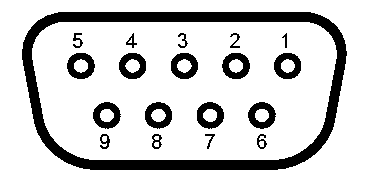
\includegraphics[width=1\textwidth]{grafiken/Numbered_DE9_female_Diagram.pdf}\\
    Front view
  \end{minipage}
  \hfill
  \begin{minipage}[b]{0.49\textwidth}
    \centering
    \begin{tabular}{cc}
      \toprule
      \textbf{Pin} & \textbf{Function} \\
      \toprule
      1 & Phase B1 \\ \midrule
      2 & Phase B2\\ \midrule
      3 & Phase A2 \\ \midrule
      4 & Phase A1 \\ \midrule
      5 & Ground \\ \midrule
      6 & +5V \\ \midrule
      7 & Sens 1 \\ \midrule
      8 & Sens 2 \\ \midrule
      9 & Sens 3 \\ \midrule
      Shield & NC \\
      \bottomrule
    \end{tabular}
  \end{minipage}
\caption[Pinout of the motor connectors.]{Pinout of the motor connectors.}
\label{pin_out}
\end{figure}

The power connector is a R7B female connector. Please refer to figure~\ref{pin_out_power} for its pinout.

\begin{figure}[h]
\begin{center}
\begin{minipage}[h]{0.49\textwidth}
    \centering
    %R7B female connector\\
    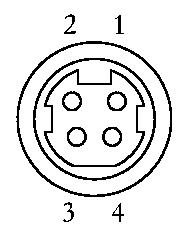
\includegraphics[width=0.55\textwidth]{grafiken/R7B.pdf}\\
    Front view
  \end{minipage}
  \hfill
  \begin{minipage}[h]{0.49\textwidth}
    \centering
    \begin{tabular}{cc}
      \toprule
      \textbf{Pin} & \textbf{Function} \\
      \toprule
      1 & + 24V \\ \midrule
      2 & Ground\\ \midrule
      3 & Ground \\ \midrule
      4 & + 24V  \\ \midrule
      Shield & NC \\
      \bottomrule
    \end{tabular}
  \end{minipage}
\end{center}
\caption[Pinout of the power connector.]{Pinout of the power connector.}
\label{pin_out_power}
\end{figure}






\newpage
